\section*{Why we care about preferences}

% If we want to understand how two states interact in international politics, we need to know how similar their foreign policy preferences are.

Understanding state interactions in the realm of international politics necessitates some knowledge of states' foreign policy preferences vis-\`{a}-vis each other.  We can consider each state to have a preferred policy outcome on each possible issue that might arise in international relations. We can conceive of these preferred outcomes as an ideal point in multidimensional space. Given the fact that many issues in international politics are related, we can represent these preferences in far fewer dimensions than there are issues in international politics. These preferences will also change over time. When states have similar preferences on an issue, they will be more likely to collaborate to achieve their joint preference on that issue, and more generally states with similar foreign policy preferences will be cooperative in a larger proportion of their interactions. States with similar preferences are also unlikely to be involved in violent disputes with each other because the policy benefits of these disputes are unlikely to surpass the cost of fighting. Conversely, when states have highly dissimilar foreign policy preferences, cooperation will be difficult and violence will be more common. Unfortunately, while we have abundant data to measure the strength of states' economies, the volume of trade between states, or even their military power, it is much more difficult to measure states' preferences, because as with many social and political constructs they cannot be observed directly.

Effectively measuring state preferences would yield scholars a number of benefits. A number of formal theories of international relations require measures of preferences to be tested: the expected utility theory proffered by \citep{buenodemesquita:1983} has similarity of preferences as an important input. Further attempts to expand studies of crisis bargaining to include mediation \citep{kydd:2003}, coalitional dynamics \citep{wolford:2014}, or the possibility of additional disputants \citep{gallop:2017} require a measure of state preferences in order to predict whether war will be the result of bargaining failure. Preferences have been used in empirical studies predicting bilateral trade, foreign aid, stability of international institutions and the incidence of conflict \citep{derouen:heo:2004, stone:2004, gartzke:2007, kastner:2007, braumoeller:2008}. 

A substantive theoretical reason for why we need a good measure of preferences is to correctly understand the democratic peace. It is difficult to entangle whether democracies avoid war with other democracies because of the intrinsic nature of democracy, or simply because they appear to share similar ends. \citet{farber:gowa:1995} argue that democracies were only peaceful during the Cold War period because they had similar preferences and alliance structures. Similarly, \citet{gartzke:1998} argues that dissimilar preferences are a necessary condition for conflict. \citet{oneal:russett:1999e} respond by arguing that democracy has both a direct inhibiting effect on conflict, and an indirect one through influencing state preferences.\footnote{\citet{gartzke:2000} argued that even though democracies might have similar preferences, the residual of preferences from democracy explains conflict much better than the residual of democracy from preferences.} While there has been some impressive development with measures of preferences in recent years, a more accurate measure is essential to disentangle the extent to which peace is the product of shared preferences, and the extent to which institutions and norms are driving peace.

%To provide this more accurate measure we take a multilayer network based approaches to estimating state preferences. Much of the extant literature has employed spatial weighting models \citep{signorino:ritter:1999,bailey:etal:2015} on relational data such as alliance behavior and UN voting scores. We make  

Much of the extant literature has focused on estimating state preferences by utilizing spatial weighting models on either alliance behavior or United Nations (UN) voting scores. These approaches have proven to be useful but there are two reasons to desire a different approach. First, alliances are rare and voting together in the UN is very common, so, by only focusing on the direct dyadic behavior, we risk mischaracterizing important relationships. Second, we would expect a better understanding of state preferences to help us predict state behavior, but as we show in Figure \ref{fig:rocShitty} adding measures of state preferences to a traditional model of interstate disputes yields relatively scant increases in terms of predictive ability.

\begin{figure}[ht]
	\centering
	\begin{tabular}{cc}
	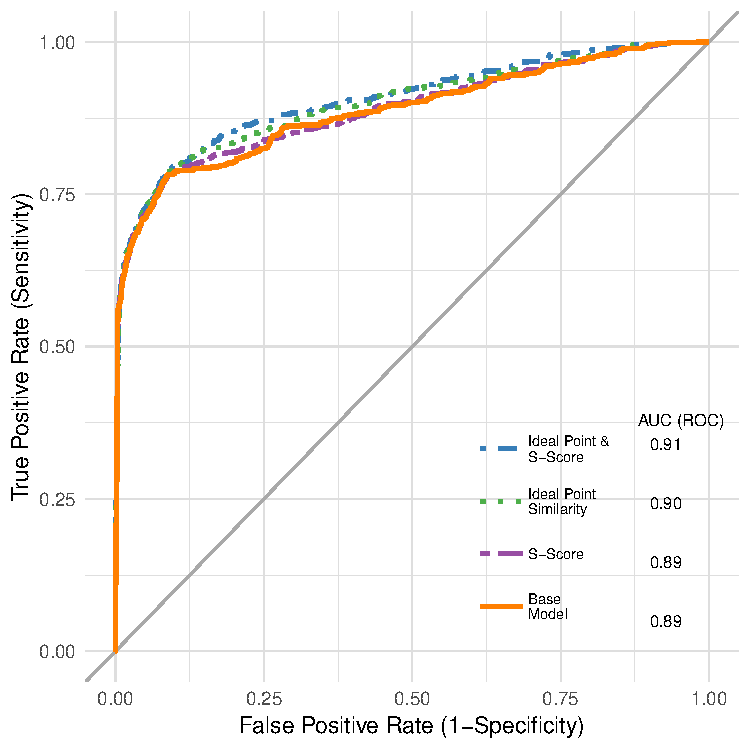
\includegraphics[width=.5\textwidth]{roc_outSample_noLatAngle.pdf} & 
	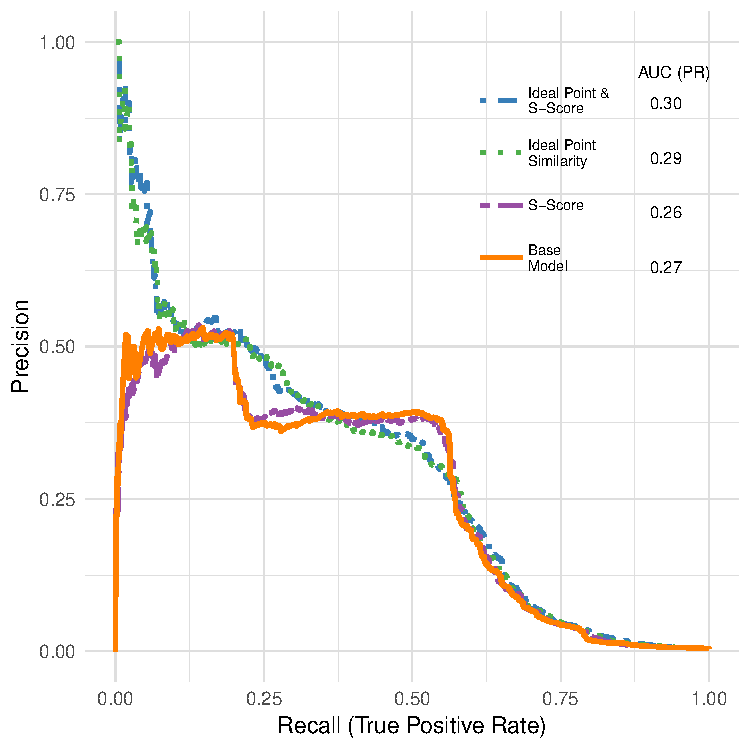
\includegraphics[width=.5\textwidth]{rocPr_outSample_noLatAngle.pdf}	
	\end{tabular}
	\caption{Assessments of out-of-sample predictive performance of Militarized Interstate Disputes using ROC curves and PR curves. AUC statistics are provided as well for both curves.}
	\label{fig:rocShitty}
\end{figure}

We can improve on these measures of preferences using the same raw material by acknowledging that both alliance membership and UN voting are layers of relationships that takes place simultaneously and in an interdependent context. Specifically, these relations between states constitute a multilayer network, in which the various layers correspond to different ways states are interacting with one another at a given time point. A bevy of research has shown that accounting for network structure necessitates an approach that can account for the indirect relations states share. As such, we make two contributions to the existing literature on state preferences. We utilize a multilinear tensor regression that enables us to measure how dependent actions of a particular dyad are across layers and time. We show that our revised approach of measuring state preferences both better characterizes relationships that have had counterintuitive results, and this measure greatly enhances our ability to predict instances of conflict.